% Koma class
\documentclass[a4paper, oneside]{scrartcl}   

\usepackage{a4wide}

%------------------
% language = english
\usepackage[english, german]{babel}	% Umlaute mit \"u
\usepackage[latin1]{inputenc}

% margins + Kopf- und Fu�zeilen
\usepackage[left = 2.5cm, right = 2.5cm, top = 2cm, bottom = 3cm]{geometry}
\usepackage{scrpage2} 
\pagestyle{scrheadings}
\clearscrheadfoot
\rehead{\headmark}
\lehead{\pagemark}
\lohead{\headmark}
\rohead{\pagemark} 


% math
\usepackage{amssymb}
\usepackage{amsmath}

% figures
\usepackage{tikz}
\usepackage{graphicx}


% section-Zaehler wird neu gesetzt:
\setcounter{section}{3}
%------------------
\author{Sascha Meiers, Martin Seeger}
\title{Exercise 7, Discrete Mathematics for Bioinformatics}
\date{Winter term 2011/2012}


\begin{document}
\maketitle

%---------------------------------------------------------------------------------------------------

\subsection{Network Flow (Niveau II)}


\subsection{Network Flow (Niveau I)}
Replace each node $v$ with its associated \emph{node capacity} $c_v$ by two new nodes 
$v_{in}, v_{out}$ and an edge $(v_{in},v_{out})$ with \emph{edge capacity} $c_v$. Then all ingoing 
edges $(u,v) \in E$ point to $v_{in}$, the outgoing edges $(v,u) \in E$ start from $v_{out}$.   


\subsection{Ford-Fulkerson}

The first figure shows the residual network according to the current flow. 
An augmenting path is marked in green.

The Ford-Fulkerson algorithm uses this path to increase the network flow by 1. 
After that the residual network as seen on the right remains. There is no augmenting path left, 
as a breadth-first search can decide. The same breadth-first search (see green arrow) 
is used to find a minimum cut (see red line), which has a capacity of 10.

\begin{minipage}[hb]{\textwidth}
\begin{center}
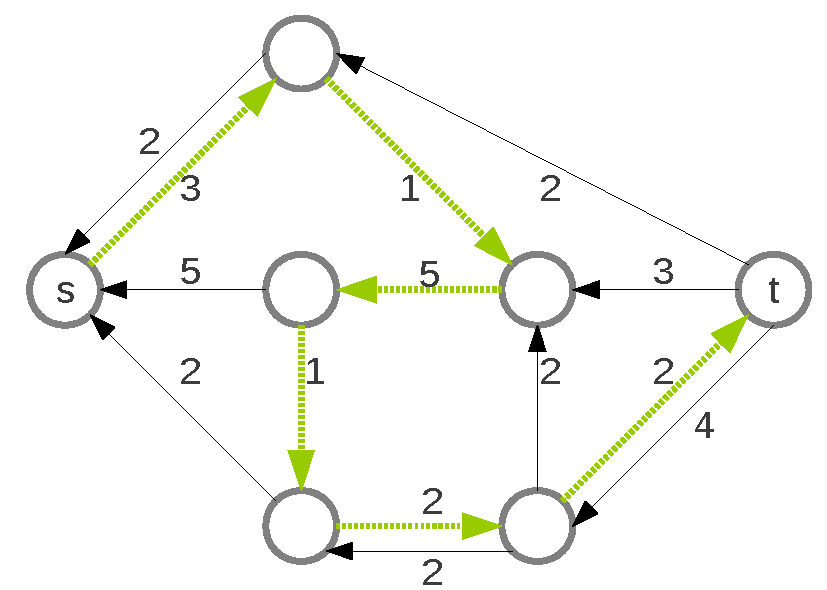
\includegraphics[width=7cm]{restnetz1.pdf}
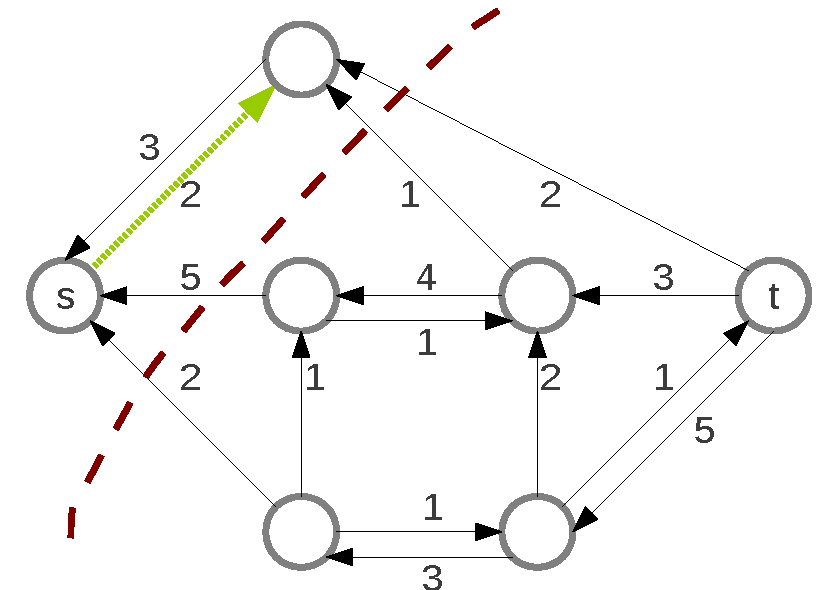
\includegraphics[width=7cm]{restnetz2.pdf}
\end{center}
\end{minipage}


\subsection{Bipartite matching}

The figure below shows the augmenting-path method to find a optimal matching in a bipartite graph.
The set of edges concerned for the matching are marked black and in each step we label a remaining 
augemting path in blue.
\begin{center}
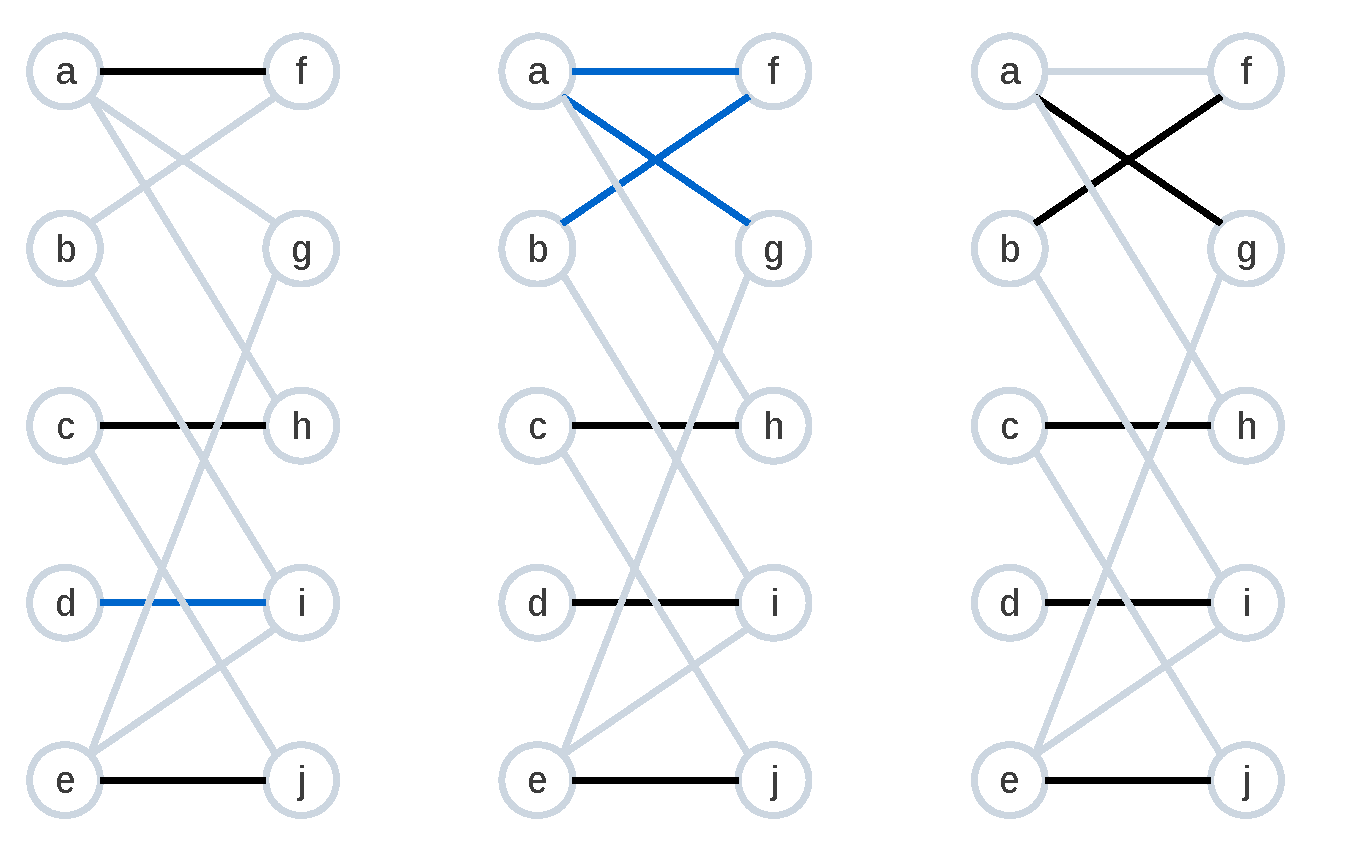
\includegraphics[width=12cm]{bipartite_matching.pdf}
\end{center}









\end{document}
